%aplicaciones

\section{Usos y Aplicaciones}

\subsection{Medicina}
% Razón de la elección.
Se diseño y aplicó una pegatina a el yeso de los pacientes de una clínica de fracturas. La etiqueta tenía un código QR, como herramientas de información y de contacto directo al elenco de la clínica para pedir ayuda o consejos. Al retirar el yeso, la gran mayoría tenía la etiqueta; los pacientes completaron un cuestionario sobre la pegatina. La gran mayoría de los pacientes, lo consideraban útil para el manejo proactivo de posibles problemas de yeso.  Otras ramas de la medicina pueden beneficiarse de la incorporación de códigos QR como fuentes de acceso a infomación.\cite{2017_Gough}
\begin{figure} 
	\centering
	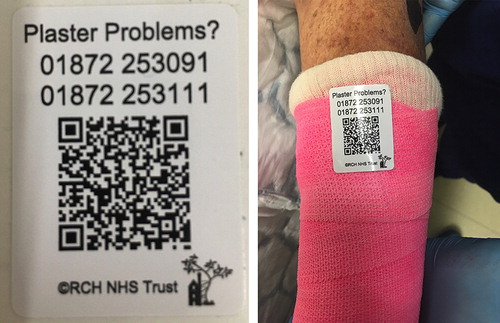
\includegraphics[width=0.5\linewidth]{rcsann.2017.0070-1.jpg}
	\caption{Código QR con fuente de información.}
	\label{fig:qryeso}
\end{figure} 
\\
COVID-19, causado por el SARS-CoV-2, se informaron oficialmente los primeros casos en diciembre de 2019; ha sido declarada pandemia mundial por la Organización Mundial de la Salud (OMS). \cite{2020_Organization} 

Para contener la propagación de enfermedades como el COVID-19, se ha empleado una variedad de enfoques de salud digital.\cite{2020_Breeher}
Uno de ellos, los códigos de salud QR basados en síntomas emitidos por las autoridades de salud pública, son cruciales porque los códigos no recuperan datos de ubicaciones. Los códigos QR se consideran oficialmente certificados electrónicos del estado de salud de las personas,y un certificado más que permitirá la entrada a otro país al dejar constancia que esa persona ha sido vacunada, siendo una medida de movilidad interna; recibiendo el nombre de pasaporte de vacunación o certificado verde digital.\cite{2020_Nakamoto,Commission2021}
\begin{figure} 
	\centering
	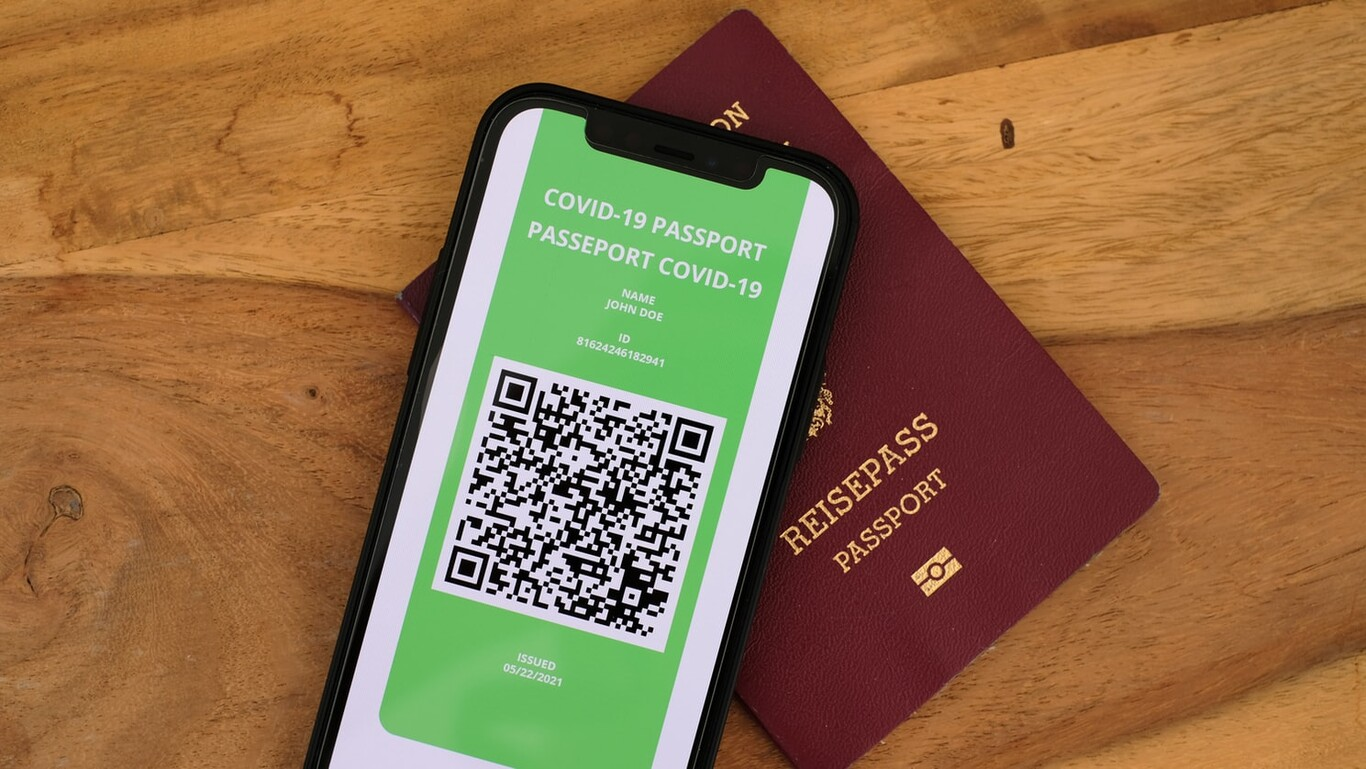
\includegraphics[width=0.5\linewidth]{qrpasaporte2.jpg}
	\caption{Código QR como pasaporte de movilidad.}
	\label{fig:qrpasaporte}
\end{figure} 


\subsection{Marketing y publicidad}
En el medio publicitario, las empresas ofrecen a los consumidores una forma de obtener información relevante de algún producto, ver opiniones de los clientes, ofrecer algún tipo de promoción; una vez que escanean el símbolo puesto en algún anuncio. Motivando el entretenimiento a lo largo de la experiencia, donde los consumidores están más involucrados con las ofertas promocionales; son especialmente importantes para los especialistas en marketing. \cite{2014_Ertekin}
\begin{figure} 
	\centering
	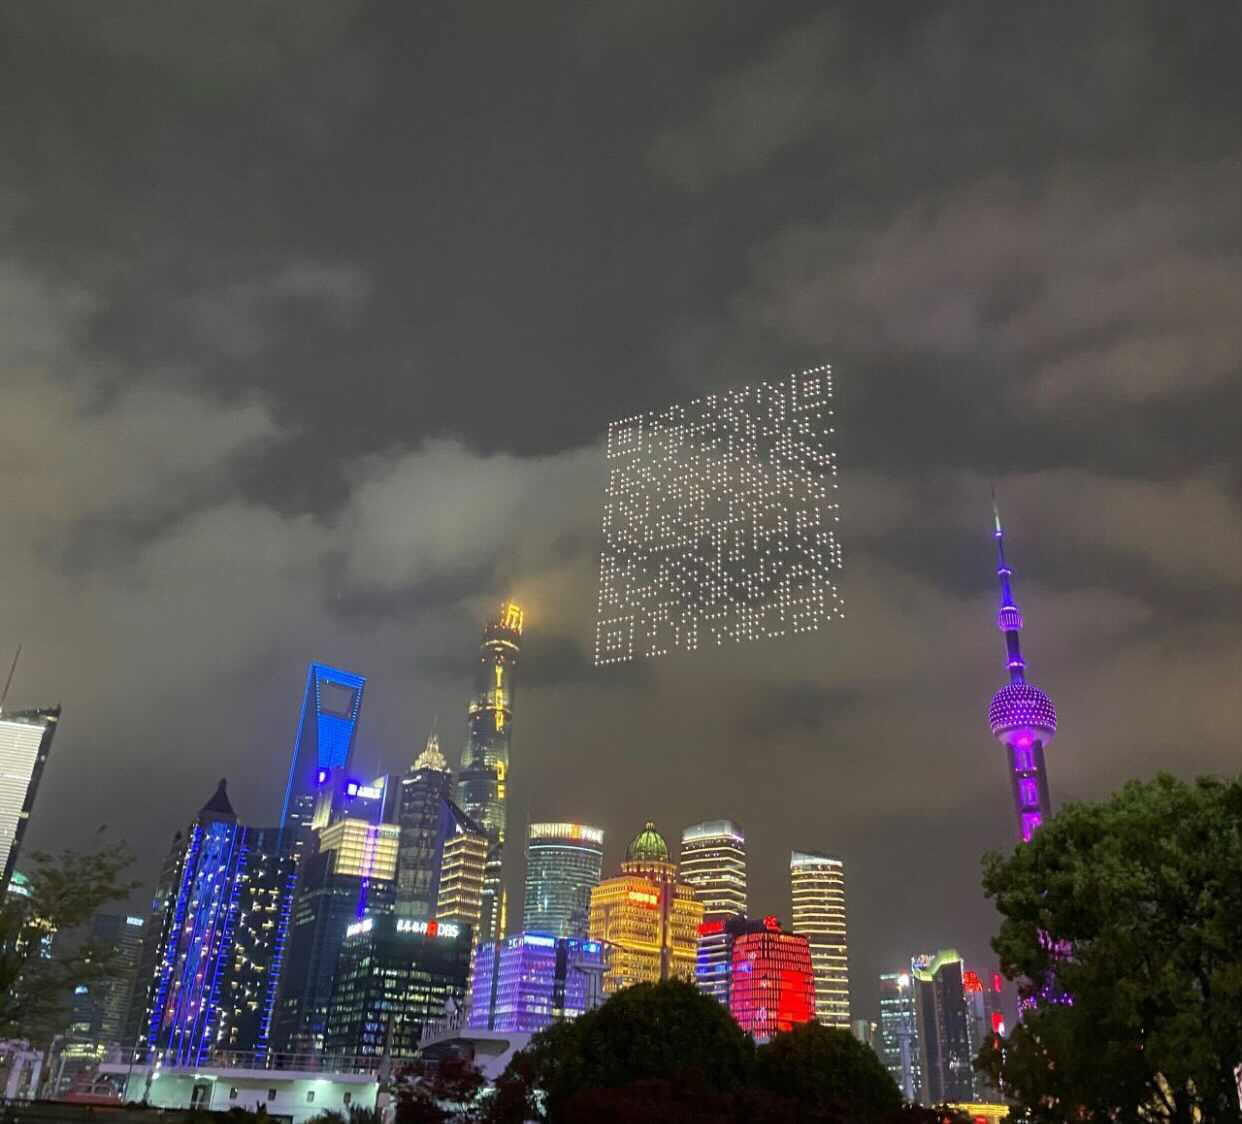
\includegraphics[width=0.5\linewidth]{qrmarketing.jpg}
	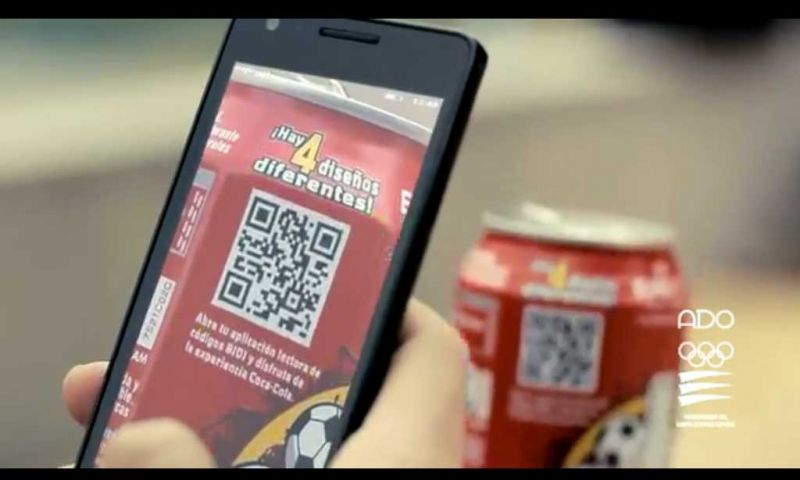
\includegraphics[width=0.5\linewidth]{anuncio-de-coca-cola-uefa-euro-2012-1.jpg}
	\caption{Código QR en Marketing}
	\label{fig:qrmarketing}
\end{figure}
\\
La empresa de bebidas Coca-Cola, fue uno de los primeros en usar los códigos QR en latas. El objetivo no era solo obtener información, busco conectar a los consumidores mediante el escaneo del símbolo, donde estos les redirigia a una página web , donde podían ver vídeos o descubrir conciertos organizados por la empresa. Siendo una buena idea de marketing orientada para los jovenes, lo que mostró el potencial de vincular lo digital con lo real.\cite{Generator2021}
Por lo tanto, pueden considerar tener juegos u otros instrumentos como incentivo para entrener a los consumidores, mediante el escaneo del código QR en anuncios. Llegando a la conclusión, de que son un sustituto factible de los cupones impresos, promociones, navegación entre pantallas y visitas físicas para investigar y obtener detalles del producto. \cite{2014_Ertekin}

\subsection{Entretenimiento}
Los museos y las galerías de arte, utilizan los códigos QR como una forma de experiencia multimedia para sus visitantes, escaneando el símbolo se puede tener una información detallada de las obras de arte, incluso videos, imágenes, audios o una combinación de ambos. Las visitas guiadas se convierten en una experiencia más interactiva, algunas galerías utilizan diferentes técnicas de presentación para atraer más visitantes. Por ejemplo, una empresa australiana, Grande Exhibitions, creó Van Gogh Alive experiencias  y el Museo de Brooklyn ha llevado el uso del código QR para la información del artista, una forma de mejorar la información sobre accesibilidad y también para mostrar el mapa del museo.\cite{2012_Emek}
\begin{figure}
	\centering 
	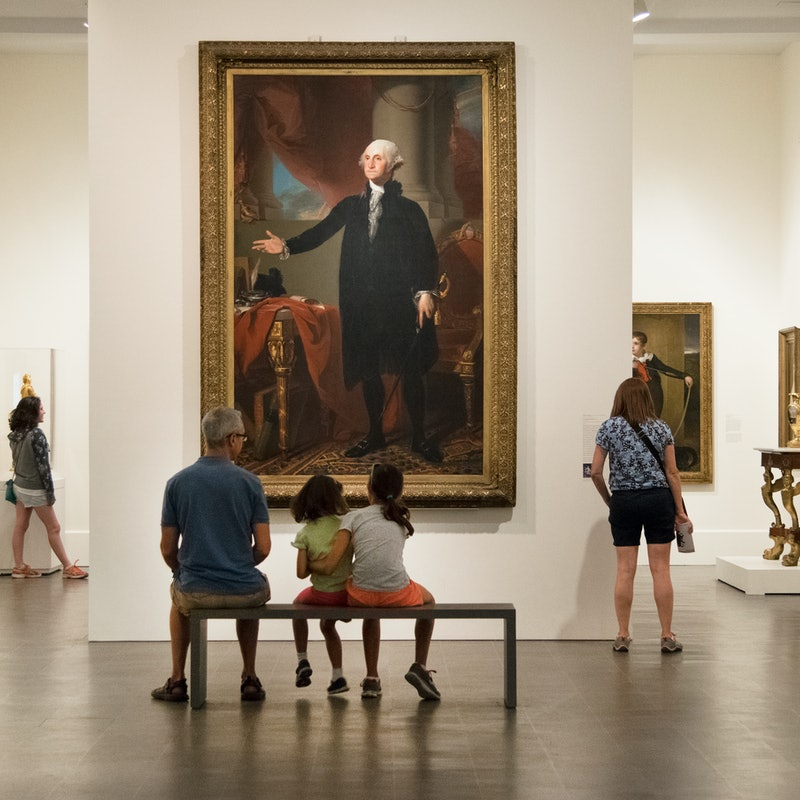
\includegraphics[width=0.4\linewidth]{museobrooklyn.jpg}
	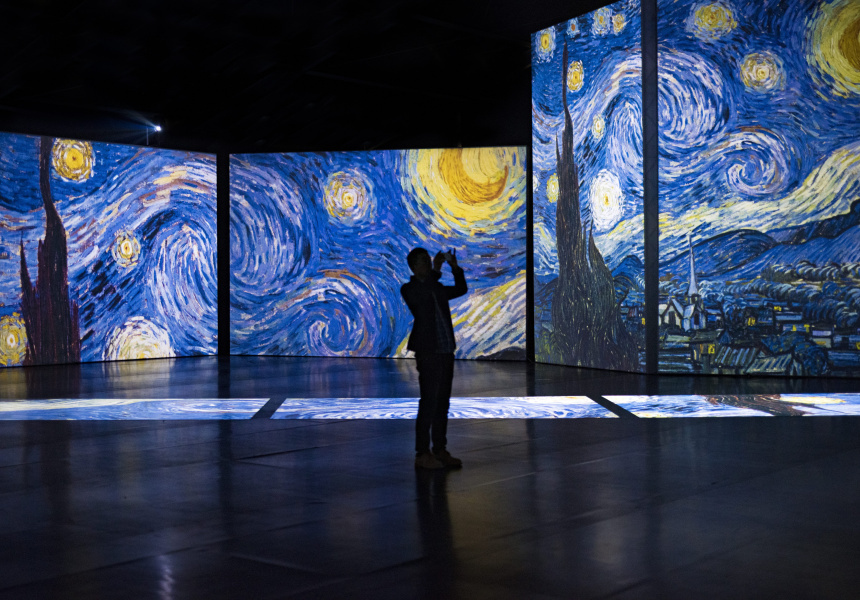
\includegraphics[width=0.4\linewidth]{vangoghalive.jpg}
	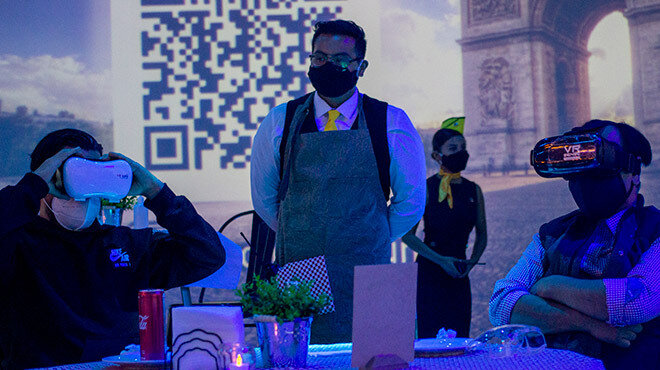
\includegraphics[width=0.4\linewidth]{vangoghalive2.jpg}
	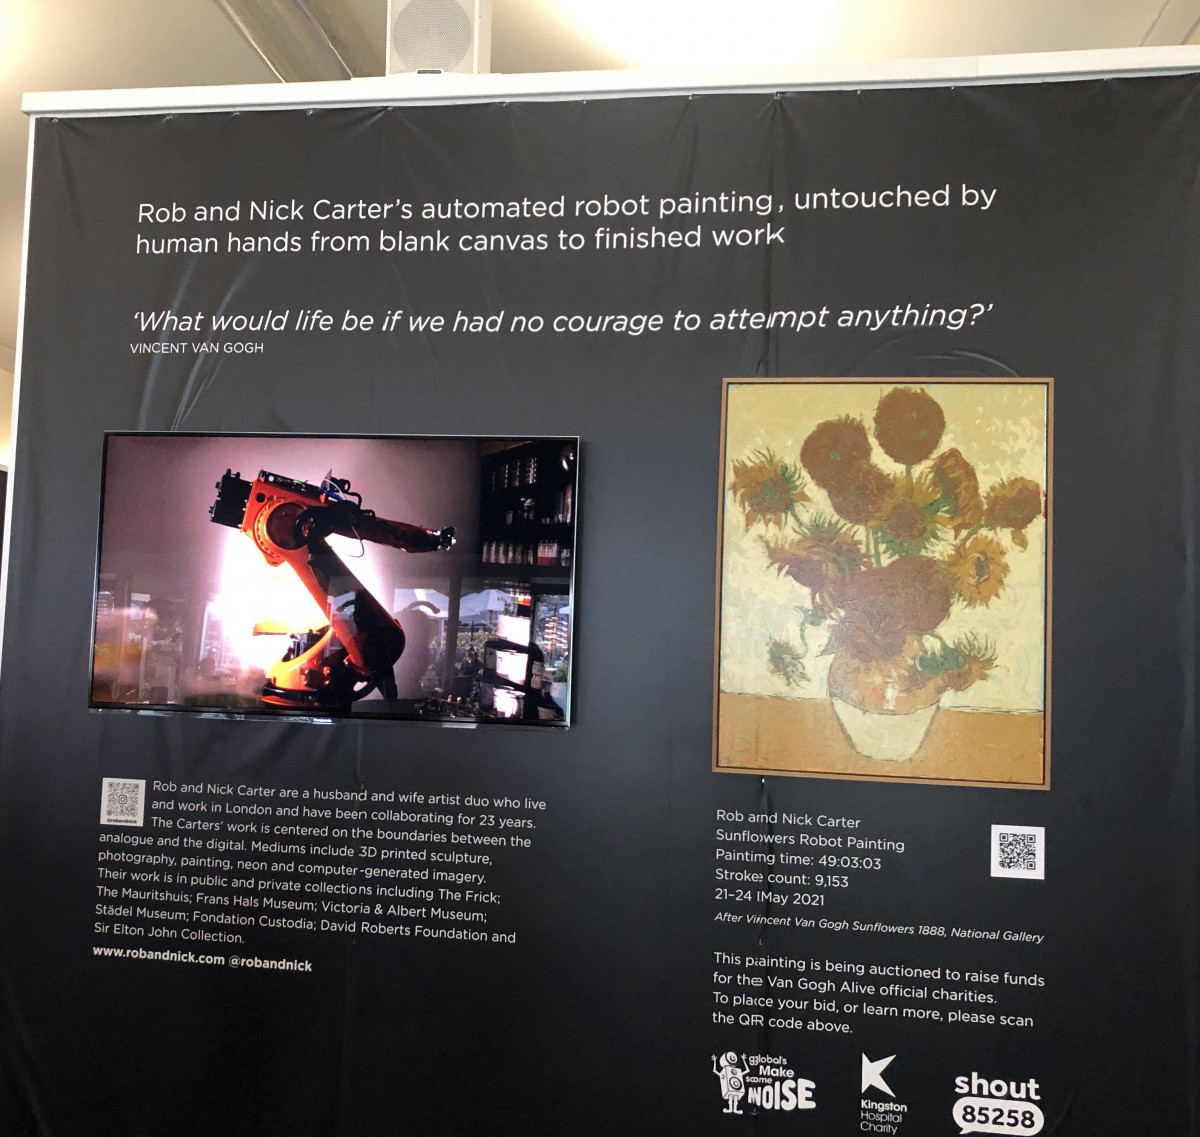
\includegraphics[width=0.4\linewidth]{vangoghalive3.jpg}
	\caption{El código QR en el entretenimiento.}
	\label{fig:qrentretenimiento}
\end{figure}

\subsection{Turismo y Transporte}

La aerolíneas utilizan el código QR para la promoción y el embarque. Por ejemplo, Securidox, incluyen un código QR en sus documentos de embarque, permitiendo redirigirlos al portal de ventas a borde de la aerolínea. Los aeropuertos pueden utilizarlos en ofertas de estacionamiento o para verificar la autenticidad del documento mediante una vía rápida. Por otra parte, es posible proporcionar información detallada sobre la zona turística, mediante el uso del símbolo QR. Mostrando itinerarios de buses, estado del tráfico de la zona, permiten conocer la historia de la ciudad, sitios patrimoniales e incluso en las carreteras. Sin duda alguna, son usados como registros -check-ins- en los hoteles, ayudando a agilizar los registros y también para recibir comentarios sobre la satisfacción de los huéspedes en los destinos.\cite{2012_Emek,2021_Vuksanovic}
%qr-code-checkin.jpg
\begin{figure} 
	\centering 
	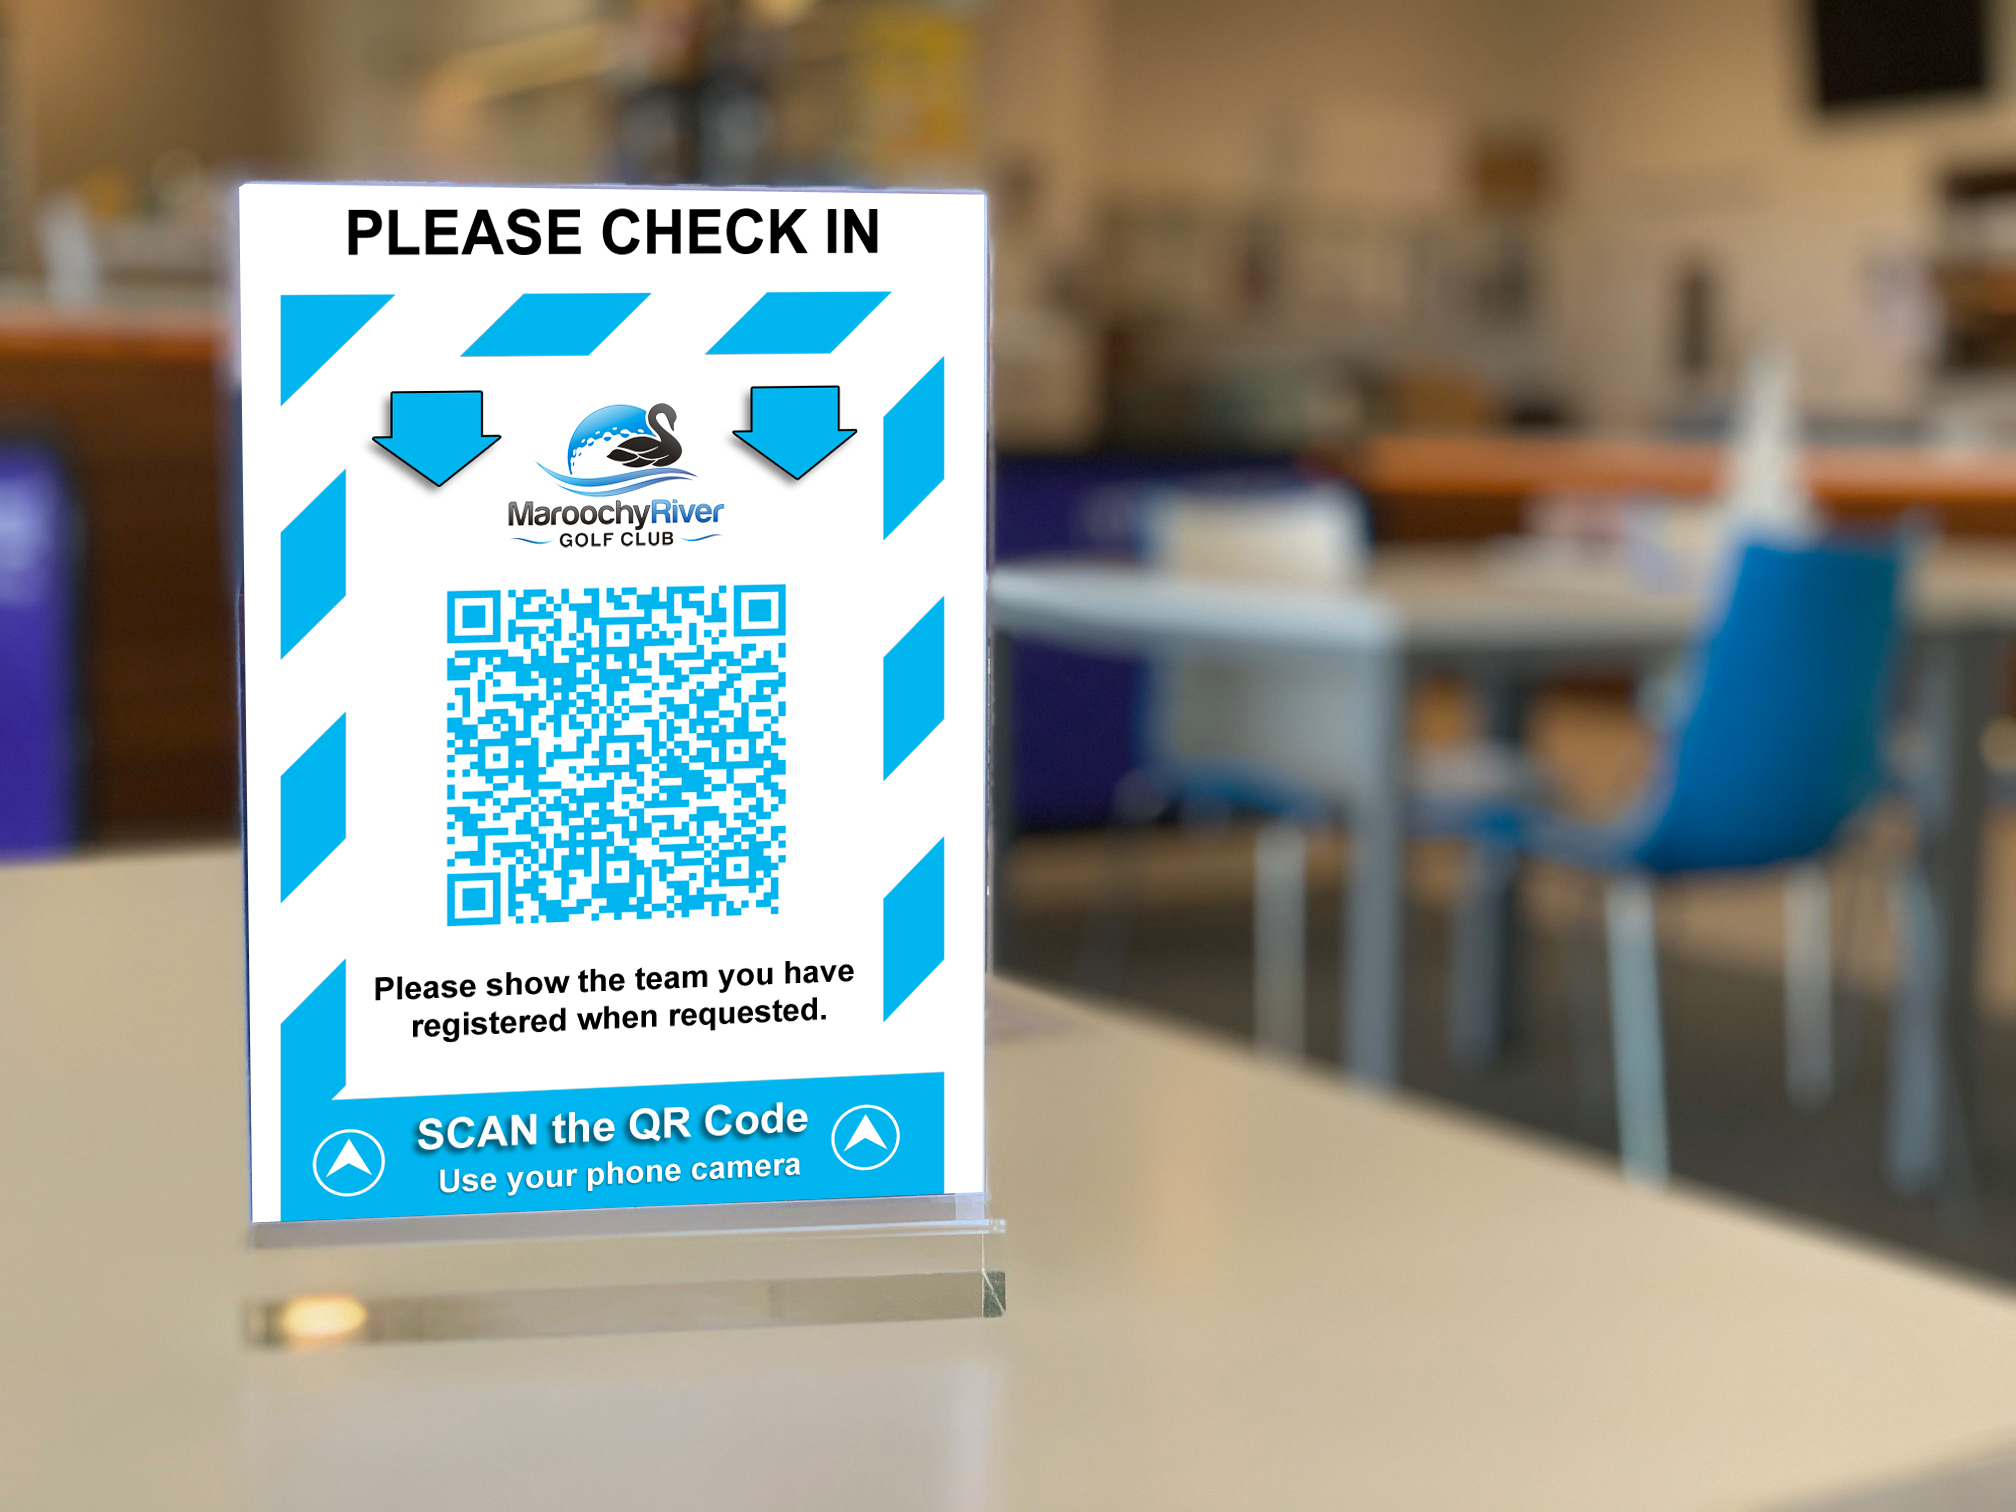
\includegraphics[width=0.3\linewidth]{qr-code-checkin.jpg}
	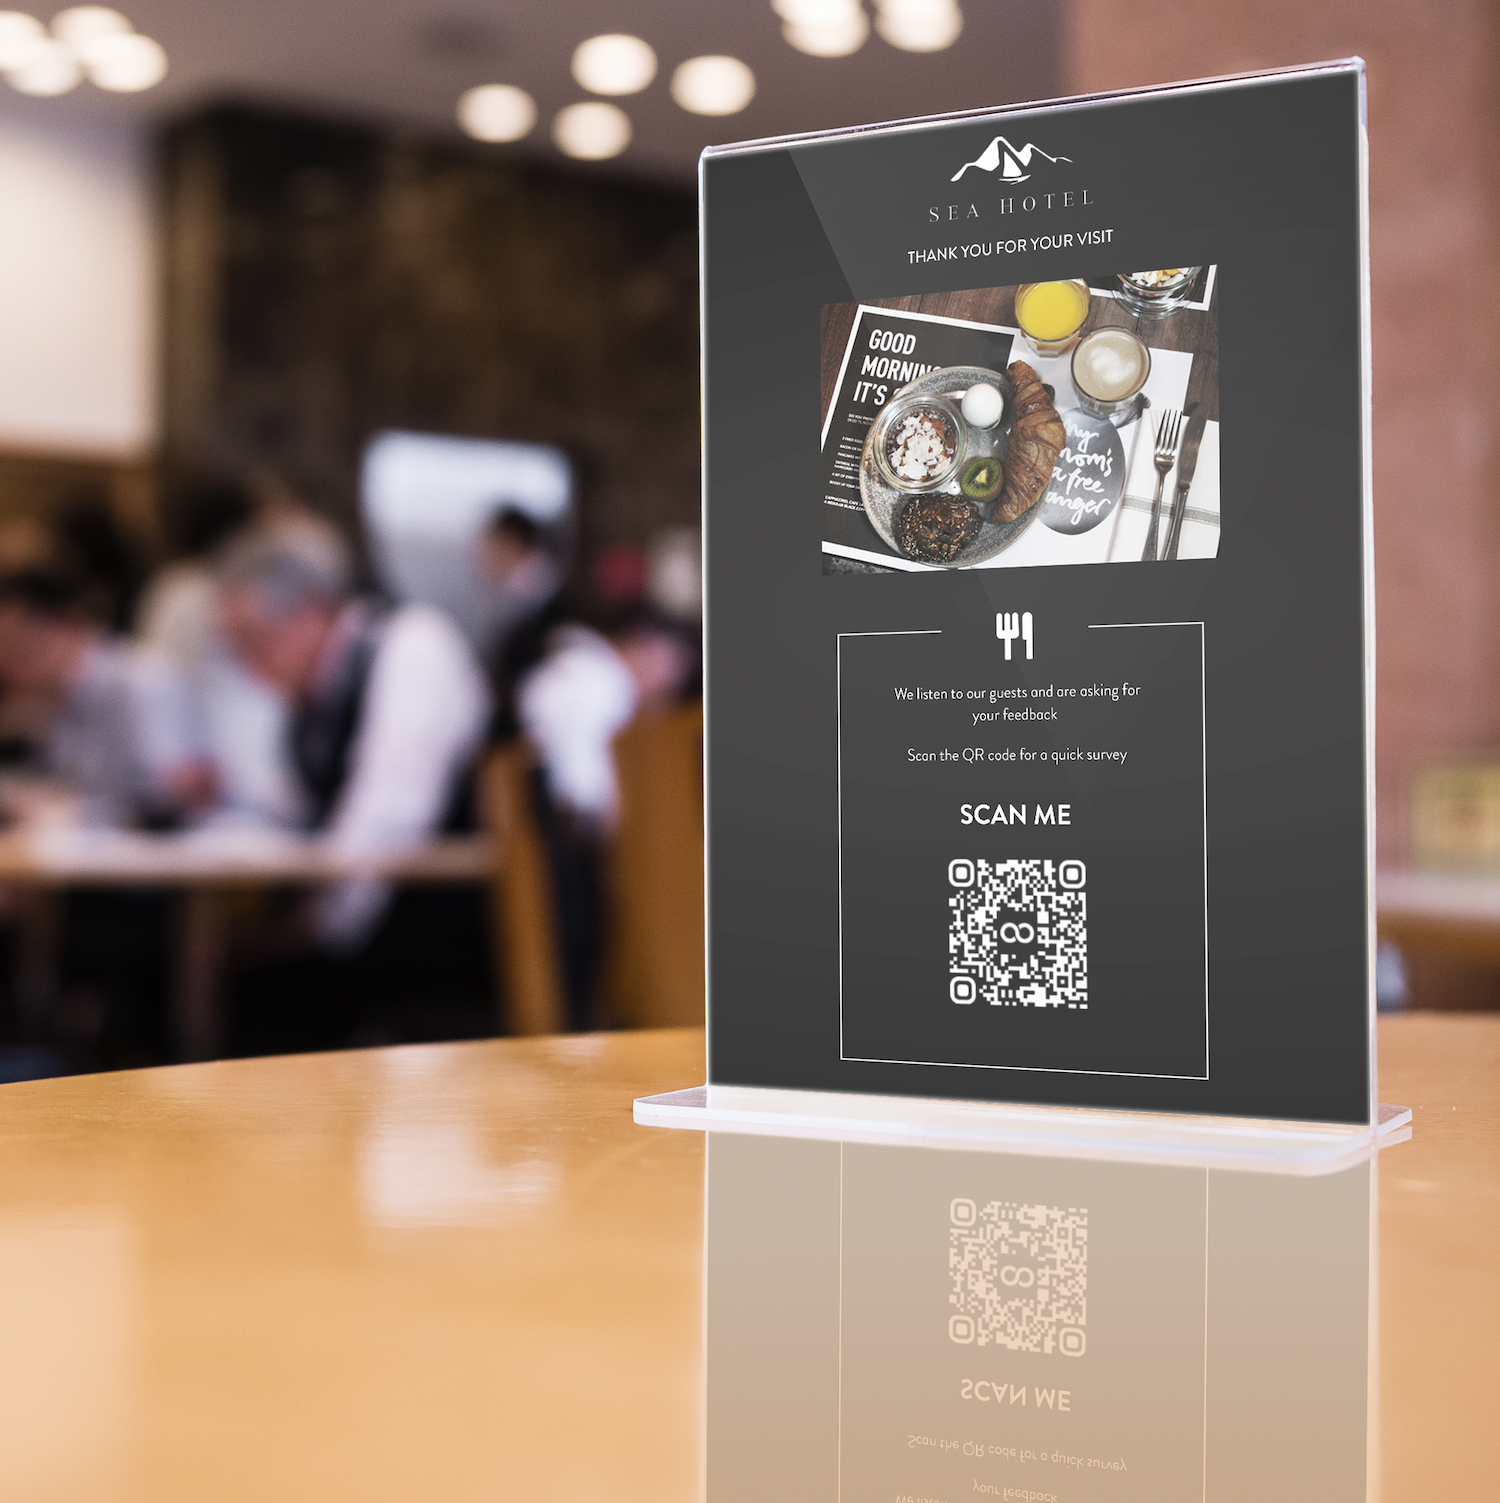
\includegraphics[width=0.3\linewidth]{qr-code-checkin2.jpg}
	\caption{El código QR en el turismo.}
	\label{fig:qrturismo}
\end{figure}

\subsection{Arquitectura y construcción}

El uso de código QR permite a las empresas de construcción y los arquitectos, a mantener los registros de capacitación de trabajadores, registros de activos y cumplir las normas de seguridad. Por ejemplo, verificar el tiempo de uso o el tiempo de vida de alguna herramienta para evitar accidentes por su deterioro en el proyecto de construcción, dado que deben seguir ciertos estándares y protocolos de calidad para garantizar la seguridad a los operadores. 
%qrconstruccion
\begin{figure} 	
	\centering
	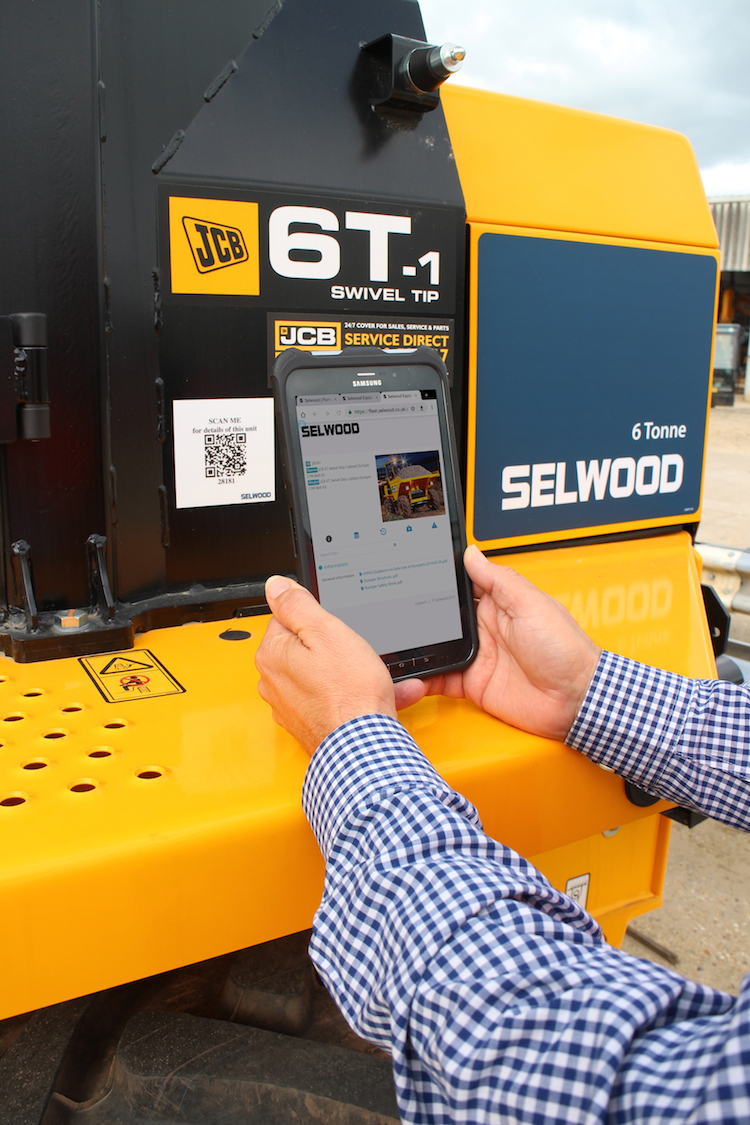
\includegraphics[width=0.2\linewidth]{qrconstruccion.jpg}
	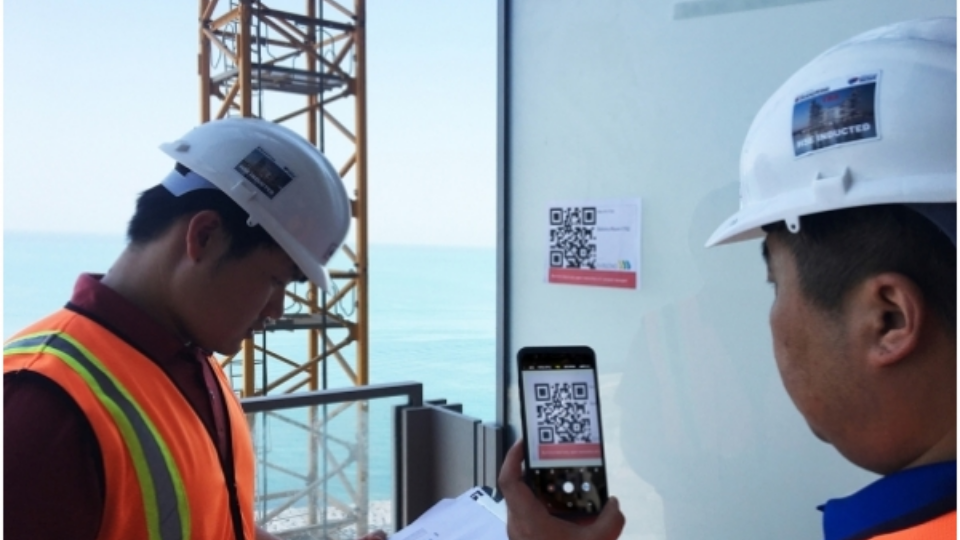
\includegraphics[width=0.4\linewidth]{qrconstruccion2.png}
	\caption{El código QR en la construcción.}
	\label{fig:qrconstruccion}
\end{figure}

El símbolo QR es utilizado para la verificación de la capacitación de los trabajadores de la construcción, para evitar lesiones, sanciones e incluso la muerte por falta de capacitación en una de las herramientas de la construcción.  Asimismo, son usados para mejorar la comprensión y simplificar el proceso de un plan de seguridad operativa o para mantenerse al día con los cambios de diseño, horarios, para evitar robos de herramientas, entre otros. \cite{delivr2021}

\subsection{Educación}
En la educación, se propuso un sistema que se ocupa de la gestión y evaluación de la asistencia de estudiantes. Donde una aplicación genera el código QR ingresando los datos del estudiante y la segunda para tomar la asistencia y generarla en formato CSV o XLS. El profesor escanea el código QR del estudiante para confirmar su asistencia, verificando la identidad del estudiante para eliminar registro falso. \cite{2017_Wei}
\begin{figure} 	
	\centering
	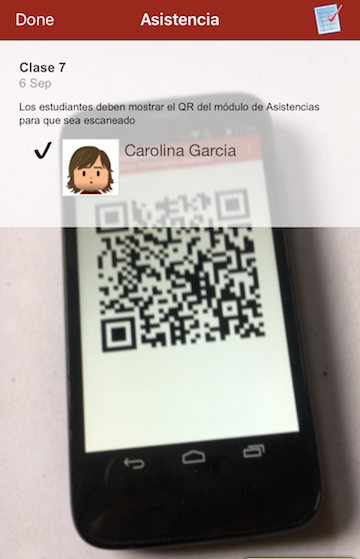
\includegraphics[width=0.2\linewidth]{asistenciaqr.png}
	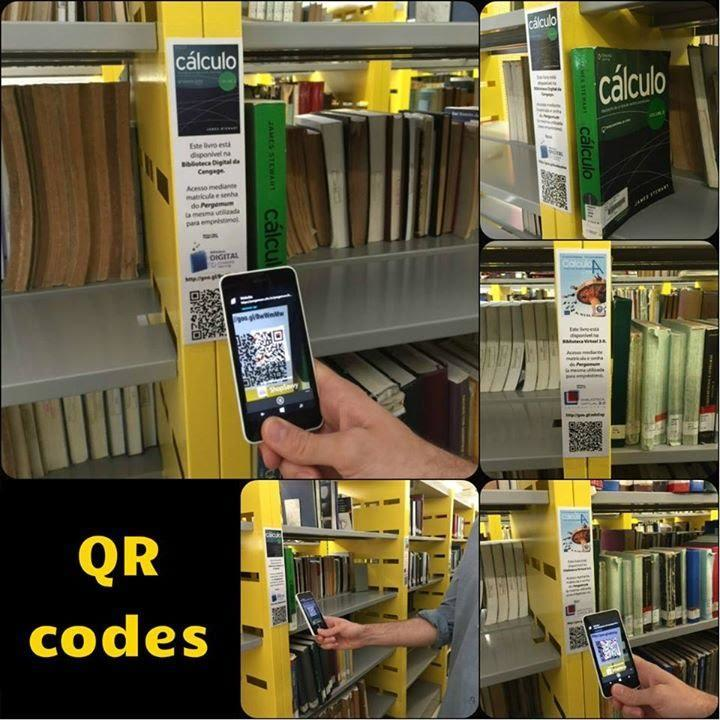
\includegraphics[width=0.3\linewidth]{qrbiblioteca.png}
	\caption{El código QR en la Educación .}
	\label{fig:qreducacion}
\end{figure}
\\
En cambio, la bibliotecas es un medio para comunicar a los usuarios sus documentos/información que desean. En el siglo XXI están completamente automatizadas, la tecnología como el código QR exige cambios en el manejo de la información en la biblioteca. El usuario mediante el uso del código QR, podra obtener información como el registro bibliográfico, añadir información básica del libro y su localización en la biblioteca.\cite{2017_Parabhoi}

\subsection{Gastronomia}
Los restaurantes utilizando la tecnología QR brindan a sus clientes información sobre el menú, la comida y bebida que se sirven, incluyendo información calórica o publicidad de porque deberian elegir su producto con respecto a la competencia. Algunos anuncios fuera del local gastronomico, podrian ofrecer descuentos en la comida o algún producto gratuito con su comida; solo para los clientes que han escaneado el símbolo QR.\cite{2012_Emek}
\begin{figure} 	
	\centering
	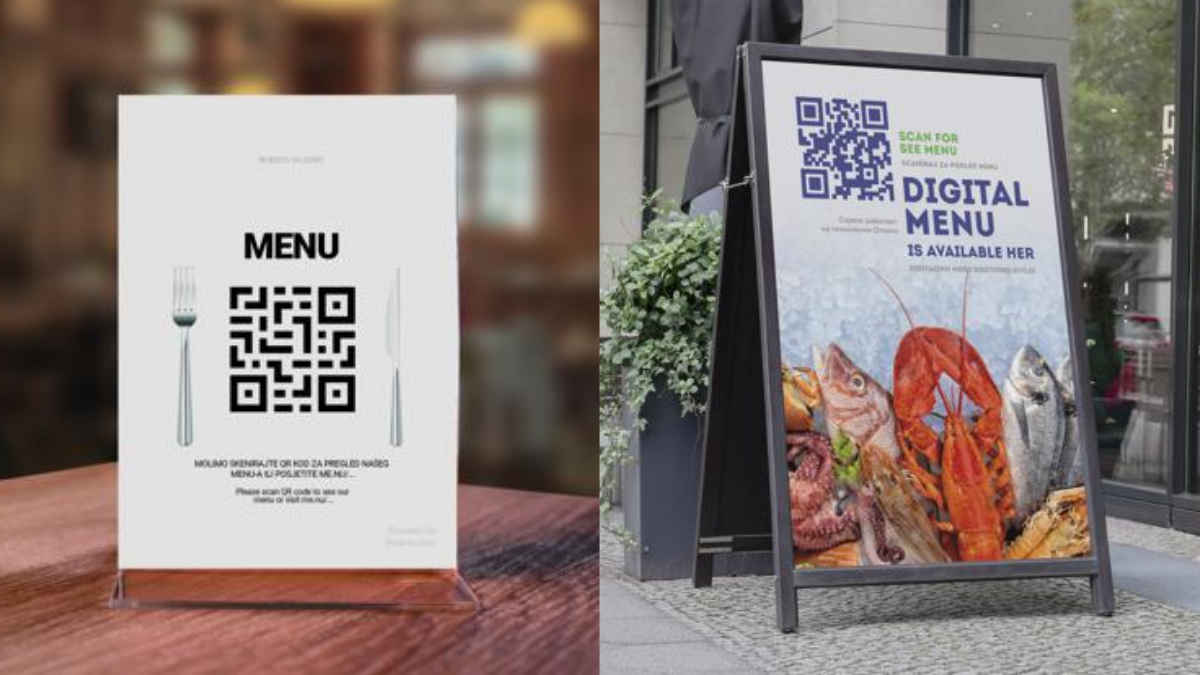
\includegraphics[width=0.6\linewidth]{qrmenu.jpg}
	\caption{El código QR en la Gastronomia .}
	\label{fig:qrmenu}
\end{figure}

\subsection{Comercio o Logística}
Con los avances en el comercio electrónico, la industria de logística no cambia mucho del transporte tradicional de mercancias, las características de lotes pequeños, velocidad y bajo costo. Al mismo tiempo, se utilizan pequeños robots como tecnología de almacenamiento flexible, ver figura (\ref{fig:datamatrixaplicaciones}). Por ejemplo, el modelo de almacenamiento flexible basado en RFID y código QR a partir del análisis de la logística. El robot planifica la ruta con estas dos tecnologías, considerando el tiempo y el conflicto de tráfico y el espacio del almacén.\cite{XiaoLong2017}
\\
Es posible realizar compras y pago por medio del escaneado del código QR, el cliente almacena sus producto en el carrito, y luego realiza el pago. \cite{2018_Banu}

\subsection{Bitcoin y Misterio-Conspiración}

El código QR es utilizado para realizar pagos con bitcoins, el símbolo contiene la ``dirección bitcoin'', que es como una dirección de correo electrónico compuesto de una larga cadenas de letras y números. Por esta razón, es utilizado para dar fácilmente su dirección a otras personas sin que tengan que escribir la larga cadena.\cite{2015_Antonopoulos_BOOK}
\begin{figure} 	
	\centering
	
\includegraphics[width=0.2\linewidth]{bitcoinQR.png}
	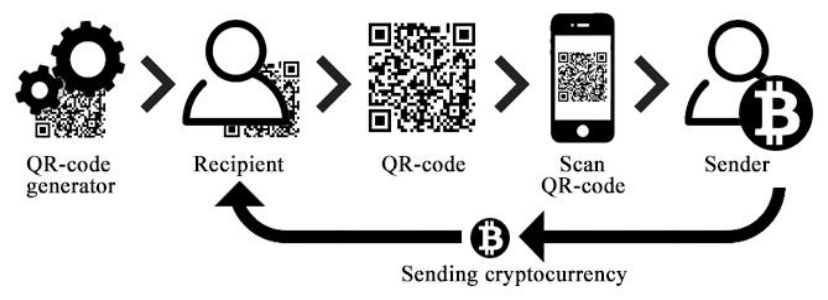
\includegraphics[width=0.5\linewidth]{Cryptocurrency-transfer-or-payment-process.png}	
	\caption{Uso del código QR, en un proceso de transferencia y pago de bitcoins.}
	\label{fig:qrbitcoin}
\end{figure}
\\
El 4 de enero de 2012, aparecio en los foros /b/- Random Board de 4chan una imagen que fue posteada por 3301, diciendo que la imagen tenía un mensaje oculto, dando comienzo a uno de los mas grandes scavengers hunt que internet hubiera tenido, a tan solo unos minutos desde que se posteo la imagen, alguien descubrio lo que la imagen contenía, adentro tenía un string leíble  y utilizando un método de descifrado, daba una dirección web que nos dirigía a otra imagen. Luego de varios desafío de la misma forma... Se llegó que la primera imagen multiplicando su altura x ancho x 3301 = 845145127, utilizando como una dirección web: www.845145127.com, la página  web tenía un contador que al finalizar mostraba unas ubicaciones conformadas con latitud y longitud alrededor del mundo, en donde cada una de las ubicaciones tenia un código QR especial, el código almacenaba una dirección web,  que te dirigía a una imagen y está imagen tenia un acertijo, y el acertijo te llevaba a un libro y el libro te llevaba a una página donde solo un limite de personas podían ingresar, luego la página web final se quedaba fuera de servicio. \cite{lemmino2018}
\begin{figure} 	
	%\centering
	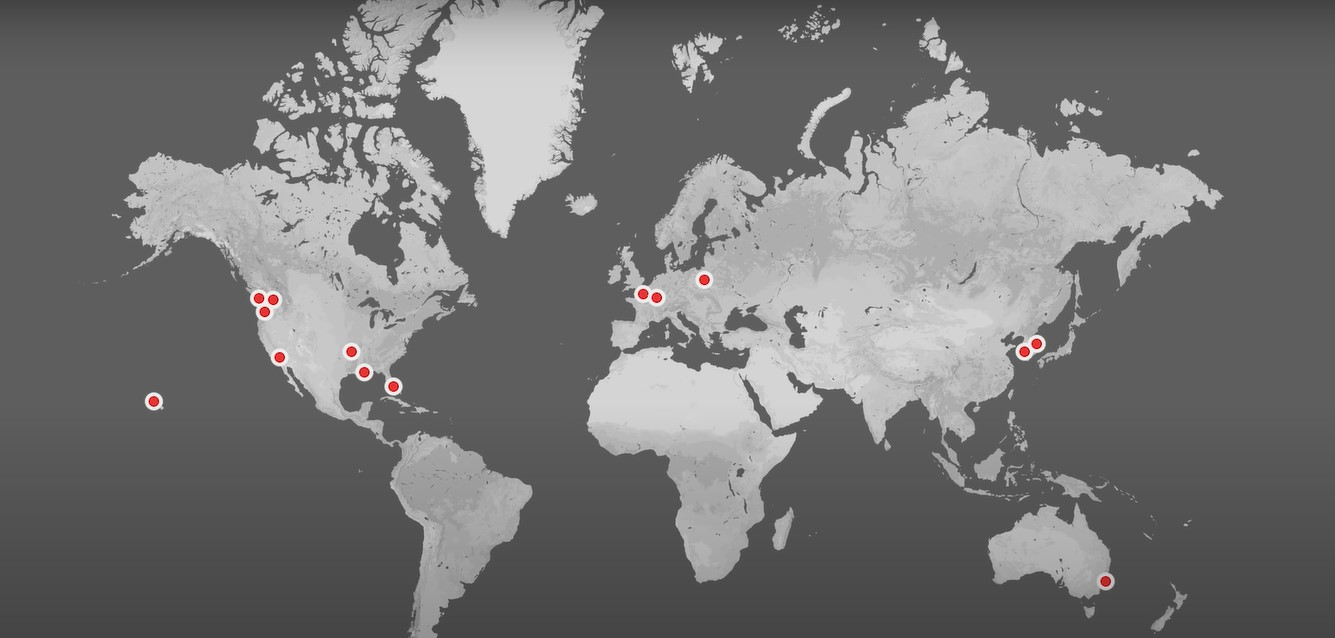
\includegraphics[width=0.9\linewidth]{cicada3301QRcodeLocations.jpg}
	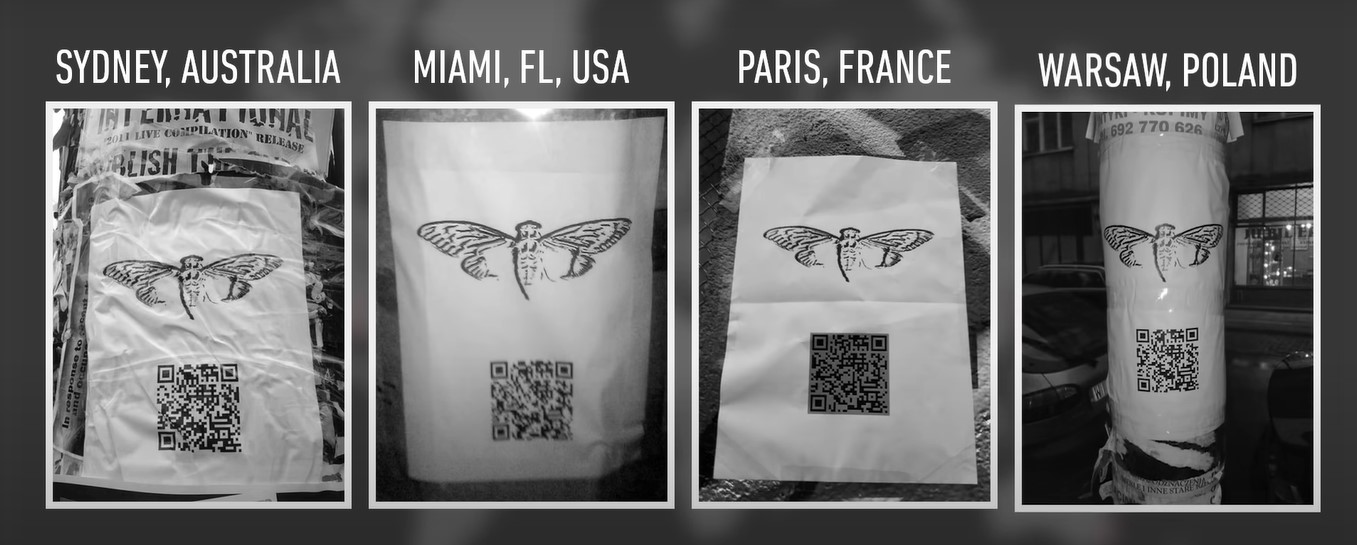
\includegraphics[width=0.9\linewidth]{cicada3301QRcode.jpg}	
	\caption{Ubicación de los Códigos QRs de cicada3301 }
	\label{fig:qrcicada3301}
\end{figure}

